\documentclass[a4paper, 11pt, titlepage]{article}
\usepackage{fancyhdr}
\usepackage{graphicx}
\usepackage{imakeidx}
\usepackage{makeidx}
\usepackage{mathtools}
\usepackage[spanish]{babel}
\usepackage{eurosym}
\usepackage{hyperref}
\usepackage{amssymb}
\usepackage{listings}
\usepackage{xcolor}
\usepackage{mathtools}
\usepackage{blkarray, bigstrut}
\usepackage{stackrel} 

\title{Tecnología de computadores}
\author{Francisco Javier Balón Aguilar}

\begin{document}

\maketitle
\renewcommand{\contentsname}{Índice}
\tableofcontents
\newpage

\section{Álgebra de Boole y puertas lógicas}

    El matemático y filósofo George Boole enunció una teoría matemática que permitía, de forma 
    algebráica, representar y operar con lógica preposicional. Una de sus características más 
    importantes es que las variables sólo podían tener dos valores: verdadero y falso. A esta 
    teoría se le conoce como Álgebra de Boole.

    Posteriormente, Claude E. Shannon, ingeniero electrónico, llega a la conclusión de que 
    es posible aplicar el Álgebra de Boole para el diseño, estudio y simplificación de circuitos 
    digitales. Uno de los factores que lo permiten son la simplificación a dos los valores de 
    las variables.

    El Álgebra de Boole queda definida, pues, por las siguientes reglas:

    \begin{itemize}
        \item Las variables sólo tienen dos posibles valores: 0 ó 1, es decir, utilizamos el 
        sistema de numeración binario.
        \item Operación de complementación o función NOT.
        \item Operación de suma lógica o función OR.
        \item Operación de producto lógico o función AND.
        \item Por convenio, el producto lógico es precedente a la suma lógica.
    \end{itemize}

    Estas operaciones algebráicas se implementan en los circuitos digitales mediante \textbf{puertas 
    lógicas}. Cada operación tiene asignada una puerta lógica.

    % TODO: poner gráfica con la representación de las puertas lógicas.

    Para representar los posibles resultados de la función lógica en función de las entradas se 
    utilizan las \textbf{tablas de verdad}. Ésta consta de una serie de columnas que representan 
    las variables de entrada y de salida, representando todas las combinaciones posibles de entradas.

    \begin{figure}[htp]
      \centering
      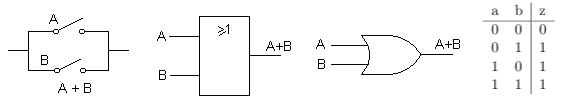
\includegraphics[width=1\textwidth]{resources/boole-or.png}
      \caption{Representación gráfica y tabla de verdad de la puerta lógica OR.}
      \label{boole-or}
    \end{figure}

    \begin{figure}[htp]
      \centering
      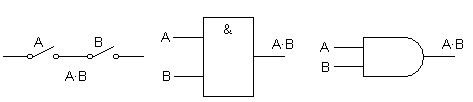
\includegraphics[width=1\textwidth]{resources/boole-and.png}
      \caption{Representación gráfica y tabla de verdad de la puerta lógica AND.}
      \label{boole-and}
    \end{figure}

    \begin{figure}[htp]
      \centering
      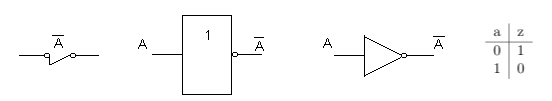
\includegraphics[width=1\textwidth]{resources/boole-not.png}
      \caption{Representación gráfica y tabla de verdad de la puerta lógica NOT.}
      \label{boole-not}
    \end{figure}

    Las puertas lógicas OR, AND y NOT son conocidas como funciones básicas (véanse figuras 
    \ref{boole-or}, \ref{boole-and} y \ref{boole-not}), cuyas operaciones cumplen las siguientes 
    propiedades:

    \begin{itemize}
      \item Conmutativa: $x+y=y+x$; $x\cdot y=y\cdot x$
      \item Elemento identidad: $x+0=x$; $x\cdot1=x$
      \item Propiedad distributiva: 
        \[x\cdot(y+x)=x\cdot y + x\cdot z\]
        \[x+(y\cdot z)=(x+y)\cdot(x+z)\]
      \item Elemento complementario: $x+\overline{x}=1$; $x\cdot\overline{x}=0$
      \item Propiedad de idempotencia: $x+x=x$; $x\cdot x=x$
      \item Elemento nulo: $x+1=1$; $x\cdot 0=0$
      \item Ley de convolución: $ \stackbin{=}{x}=x$
      \item Ley de absorción: $x+x\cdot y=x$; $x\cdot(x+y)=x$
      \item Propiedad asociativa: $x+(y+z)=(x+y)+z$; $x\cdot(y\cdot z)=(x\cdot y)\cdot z$
      \item Teorema del consenso:
        \[xy+\overline{x}z=xy+\overline{x}z+yz\]
        \[(x+y)(\overline{x}+z)=(x+y)(\overline{x}+z)(y+z)\] 
      \item Teorema de Morgan:
        \[\overline{x+y}=\overline{x}\cdot\overline{y}\]
        \[\overline{x\cdot y}=\overline{x}+\overline{y}\]
        \[x+\overline{x}y=x+y\]
        \[x\cdot(\overline{x}+y)=xy\]
    \end{itemize}

    Hay otras funciones que pueden realizarse como combinación de las funciones básicas, 
    siendo muy útiles en el diseño de circuitos digitales. Estas funciones son denominadas
    \textbf{funciones no básicas} (véanse figuras \ref{boole-nor}, \ref{boole-nand} y 
    \ref{boole-xor}).

    \begin{figure}[htp]
      \centering
      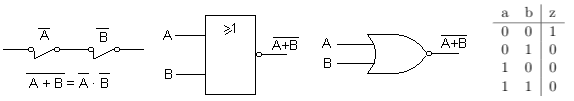
\includegraphics[width=1\textwidth]{resources/boole-nor.png}
      \caption{Representación gráfica y tabla de verdad de la puerta lógica NOR.}
      \label{boole-nor}
    \end{figure}

    \begin{figure}[htp]
      \centering
      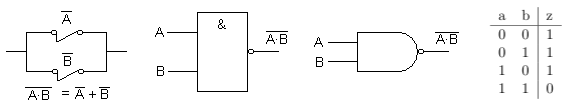
\includegraphics[width=1\textwidth]{resources/boole-nand.png}
      \caption{Representación gráfica y tabla de verdad de la puerta lógica NAND.}
      \label{boole-nand}
    \end{figure}

    \begin{figure}[htp]
      \centering
      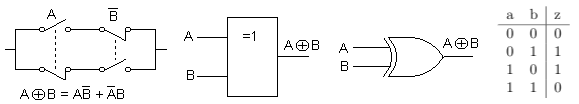
\includegraphics[width=1\textwidth]{resources/boole-xor.png}
      \caption{Representación gráfica y tabla de verdad de la puerta lógica XOR.}
      \label{boole-xor}
    \end{figure}

	\subsection{Forma canónica de las funciones lógicas}

		A partir de una función lógica podemos, mediante operaciones algebráicas, obtener 
		otras funciones lógicas equivalentes. O lo que es lo mismo, una función lógica puede 
		expresarse algebráicamente de muchas formas, siendo una de ellas la forma canónica.

		\subsubsection{Suma de minterms}

			La forma canónica de una función lógica expresada como suma de minterms\footnote{
				Un \textit{minterm} es un producto de todas las variables (negadas o sin negar)
				de una función lógica.

				Para saber si un \textit{minterm} va negado o no debemos observar si la entrada 
				es 0 ó 1; si es 0 la variable estará negado mientras que si es 1 la variable no 
				estará negada.
			} contiene la suma de todas las combinaciones de las entradas de tal forma que 
			la salida sea igual a 1.

		\subsubsection{Producto de maxterms}

			La forma canónica de una función lógica expresada como un producto de maxterms\footnote{
				Un \textit{maxterm} es una suma de todas las variables (negadas o sin negar) 
				de una función lógica.
			} contiene el producto de todas las combinaciones de las entradas que van a hacer que 
			la salida sea 0.

	\subsection{Simplificación de funciones lógicas}

		La simplificación consiste en la búsqueda de la función lógica que minimice el uso 
		de puertas lógicas. Una de las posibilidades consiste en utilizar los teoremas anteriormente 
		vistos.

		Ejemplo:
		\begin{gather*} 
			D = \overline{B}C + \overline{A}BC + ABC + \overline{A}B\overline{C} \\ 
			D = \overline{B}C + \overline{A}B\overline{C} + BC(\overline{A} + A) \\
			D = \overline{B}C + \overline{A}B\overline{C} + BC \\
			D = \overline{A}B\overline{C} + C(\overline{B} + B) \\
			D = \overline{A}B\overline{C} + C \\
			D = \overline{A}B+ C
		\end{gather*}

		\subsubsection{Homogeneización de puertas}

			Es posible implemnentar cualquier función lógica utilizando únicamente las puertas 
			NAND y NOR.
    
		\subsubsection{Mapas de Karnaugh}

			Los mapas de Karnaugh permiten simplificar funciones lógicas de una forma gráfica, sencilla 
			y sistemática, representando en una tabla (mapa) con características de la tabla de verdad de 
			una función. Debe tener las siguientes características:

			\begin{enumerate}
				\item Las posibles combinaciones de variables de entrada se colocan en filas y columnas. 
				Entre las combinaciones de entradas de dos filas o dos columnas consecutivas no debe 
				variar más de un bit.
				\item En cada celda de la tabla resultante debemos colocar el valor de la función lógica 
				para la combinación de entradas correspondientes. 
			\end{enumerate}

\section{Circuitos combinaciones}

	\subsection{Diseño de circuitos combinacionales}

		Los circuitos combinacionales son aquellos en los que las salidas sólo dependen de las entradas del 
		mismo instante. El proceso de diseñó consta de las siguientes etapas:

		\begin{enumerate}
			\item Construcción de la tabla de verdad para la función lógica que se pretende implementar.
			\item Simplificación de tabla previamente construida.
			\item Implementación de la función.
		\end{enumerate}

		Una línea de control permite que, en función del valor de las entradas el circuito se comportará de 
		una forma u otra. En función del nivel de la señal que se escoja para establecer la activación o no de 
		un determinado comportamiento, existen dos tipos de líneas de control:

		\begin{itemize}
			\item Activas a bajo nivel (cero lógico). El valor de la línea es 0.
			\item Activas a alto nivel (uno lógico). Es valor de la línea es 1.
		\end{itemize}

	\subsection{Circuitos airitméticos}

		Las operaciones aritméticas son fundamentales en cualquier computador, siendo parte importante del procesamiento de 
		la información. Los circuitos que realizan operaciones de este tipo son conocidos como circuitos aritméticos y son 
		parte fundamental de las unidades aritmético-lógicas, que forman a su vez parte de las CPUs. Estas operaciones se 
		realizan en binario.

		\subsubsection{Sumadores}

			La suma es la operación más importante de la aritmética binaria, basándose el resto de operaciones en ella.

			\[0 + 0 = 0\]
			\[0 + 1 = 1\]
			\[1 + 0 = 1\]
			\[1 + 1 = 10\]

			En ésta última el resultado es 0 y se produce un acarreo, que posteriormente se procesará, almacenará o desechará.

			\paragraph{Semisumador binario} La función del semisumador es sumar dos bits de entrada ($A$ y 
			$B$), generar una suma ($S$) y un acarreo de salida ($C_{out}$).

			\paragraph{Sumador completo} Un sumador completo tiene tres entradas, siendo la tercera la posibilidad 
			de sumar una erntrada de acarreo $C_{in}$. Esta entrada adicional permite encadenar varios sumadores, de 
			tal forma que se implementan sumadores de más de un bit; el acarreo vendría a sumar el bit anterior.

			\paragraph{Sumador de más de un bit} Para implementar la suma de números binarios se requieren tantos 
			sumadores completos como bits tengan los números que se quieren sumar, ya sea mediante acarreo 
			serie\footnote{
				El acarreo resultante de la suma de un bit se utiliza como entrada para el sumador del bit de 
				orden superior. De tal forma que para calcular la suma del bit de orden $n$ sea necesario completar 
				la suma de los $n-1$ anteriores bits. 

				Por eso, estos sumadores son poco escalables, ya que cuantos más bits tengamos, más lento será el sumador.
			} o acarreo anticipado.

		\subsubsection{Restadores}

			Para restar en binario debemos considerar las combinaciones posibles:

			\[0 - 0 = 0\]
			\[0 - 1 = 1\]
			\[1 - 0 = 1\]
			\[1 - 1 = 0\]

			En el caso de $0 - 1$ obtendremos un acarreo.

		\subsubsection{Multiplicaciones y divisiones}

			Antiguamente, la multiplicación y división se obtenía en descomposición del problema en 
			sumas y restas, con el consiguiente aumento de tiempo de cálculo. Actualmente se incluyen 
			circuitos específicos que realizan estas operaciones aritméticas. 
			
			Estos circuitos pueden ser combinacionaleso secuenciales.

	\subsection{Comparadores}

		La comparación de magnitudes se realiza mediante un circuito lógico denominado comparador.

		Un número en formato binario se introduce en la entrada $A$ y otro en la entrada $B$. Las salidas 
		$E$, $G$ y $L$ indican la relación entre los dos números, produciendo un nivel alto en la línea 
		de salida correspondiente; $E = 1$ si $A = B$, $G = 1$ si $A > B$ y $L = 1$ si $A < B$. 

	\subsection{Unidades aritmético-lógicas}

		La unidad aritmético-lógica (ALU) es un circuito combinacional capaz de realizar una amplia serie de 
		operaciones aritméticas y lógicas entre dos palabras de $n$ bits. El tipo de operaciones a realizar 
		entre ambas palabras es elegido mediante unas entradas de control de la ALU.

		\begin{figure}[htp]
			\centering
			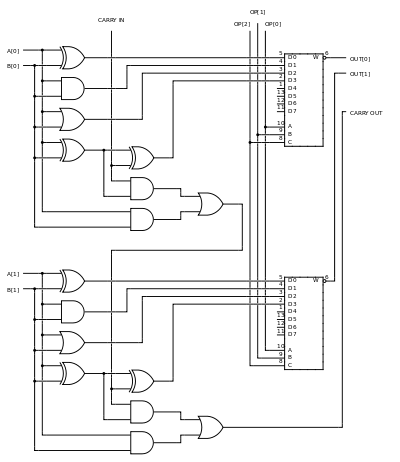
\includegraphics[width=0.7\textwidth]{resources/alu2bits.png}
			\caption{Unidad aritmético-lógica de dos bits.}
			\label{alu2bits}
		\end{figure}

		La figura \ref{alu2bits} representa una ALU de dos bits. Las entradas $A0$ y $B0$ se corresponden 
		con el bit menos significativo de los números de entrada; a diferencia de las entradas $A1$ y $B1$, 
		que corresponden con el bit más significativo.

		Las entradas $A$ y $B$ se dirigen hacia las cuatro puertas: XOR, AND, OR y XOR. Por último se realiza 
		una multiplexación para seleccionar la salida de qué operación se quiere dar como salida de la ALU. 
		La entrada $OP0-2$ determina cuál de las funciones se van a realizar:

		\begin{itemize}
			\item $OP = 000 \Rightarrow XOR$
			\item $OP = 001 \Rightarrow AND$
			\item $OP = 010 \Rightarrow OR$
			\item $OP = 011 \Rightarrow $ Suma
		\end{itemize}
  
		Estas entradas son las líneas de control de la ALU y sirven para seleccionar qué operación queremos que 
		realice.

	\subsection{Generadores y comprobadores de paridad}

		La paridad es un método de validación de la información codificada en binario. Consiste en añadir 
		un bit que hace que el número de 1s que aparece en la información sea par (paridad par) o impar 
		(paridad impar). Por ejemplo, en caso de utilizar paridad par:

		\[00110100 \rightarrow 001101001\]
		\[10011100 \rightarrow 100111000\]

		Y en el caso de utilizar paridad impar:

		\[00110100 \rightarrow 001101000\]
		\[10011100 \rightarrow 100111001\]

		De esta forma podemos detectar un error en la información, si este error se produce en un único bit y 
		sólo permite detectar errores, no corregirlos.

		Este tipo de comprobación suele usarse en transmisiones de información seguras; o de almacenamiento de 
		información (en memoria principal, por ejemplo) al que quiere dotársele de una seguridad muy alta:

		\[00110100 \xrightarrow[]{\text{paridad par}} 001101001 \xrightarrow[]{\text{transmisión}} 00110001 \rightarrow err\] 

		Sin embargo, hay que tener en cuenta que si hay un error en más de un bit puede no haber detección:
		
		\[00110100 \xrightarrow[]{\text{paridad par}} 001101001 \xrightarrow[]{\text{transmisión}} 001100101 \rightarrow ok\] 


\end{document}